\documentclass[10pt,a4paper]{article}
\usepackage[utf8]{inputenc}
\usepackage[italian]{babel}
\usepackage{amsmath}
\usepackage{amsfonts}
\usepackage{amssymb}
\usepackage{graphicx}
\usepackage{gensymb}
\usepackage[left=2cm,right=2cm,top=2cm,bottom=2cm]{geometry}
\newcommand{\rem}[1]{[\emph{#1}]}

\author{Gruppo BN \\Lisa Bedini,  Federico Belliardo, Marco Costa}
\title{Esperienza 13: Semaforo}

\begin{document}
\maketitle

%TODO - Secondo me in tutta la relazione le immagini non sono il massimo avrei voluto mettere le immagini del flip-flop congelato, ma non le abbiamo prese. Le immagini che mostrano le misure dei tempi non sono il massimo. Io le toglierei.

\section{Scopo dell'esperienza}
Lo scopo dell'esperienza � di realizzare un semaforo come macchina a stati finiti tale che
\begin{itemize}
\item nello stato ENABLED esegua un ciclo in cui si abbiano accesi (per la durata di un colpo di clock e nel seguente ordine) Led verde, Led verde e giallo, Led rosso.
\item nello stato NOT ENABLED faccia lampeggiare il Led giallo (sincronamente  col clock.
\end{itemize}
Il semaforo va realizzato sia tramite circuiti integrati, sia programmando Arduino.

\section{Materiale a disposizione}
%correggi
\begin{itemize}
\item SN74LS00 Quad NAND gate
\item SN74LS94 4-bit binary counter
\item SN74LS74 Dual D-Latch
\item SN74LS86 Quad XOR gate
\item DIP switch
\item 4 LED
\end{itemize}
%I valori delle componenti sono state misurate con multimetro digitale (incertezza riportata sul manuale).
%Le differenze di potenziale sono state misurate tramite oscilloscopio, se non indicato diversamente, e come incertezza si � presa la sensibilit� dei cursori pi� il 3\% di calibrazione.
%Per misurare i tempi si � usato l'oscilloscopio e come relativa incertezza si � preso il massimo fra la sensibilit� dei cursori e la semidispersione dei valori plausibili.

\section{Stato Enabled}
%figura circuito con piedini numerati
Per realizzare il solo stato enabled abbiamo optato per una macchina di Moore non essendoci alcun tipo di input. In figura \ref{fig:FSMenabled} abbiamo disegnato le transizioni e la codifica dei vari stati. Abbiamo deciso di usare solo 2 FF in quanto due bit erano sufficienti per codificare i tre stati richiesti. Indicheremo SEMPRE (anche nei punti successivi della relazione) $Q_2$ il bit pi� significativo, mentre $Q_1$ sar� sempre il bit meno significativo.
\begin{figure}[!htb]
\centering
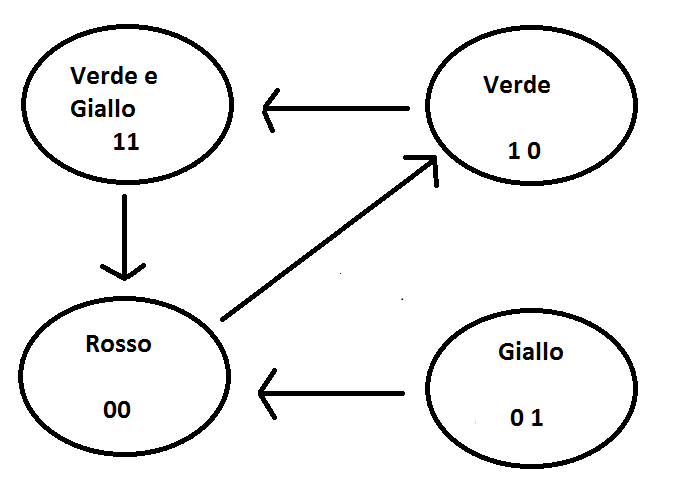
\includegraphics[scale=0.7]{FSMenabled.png}
\caption{Diagramma dello stato Enabled\label{fig:FSMenabled}}
\end{figure}
%In arrivo ftrase ambigua
Abbiamo codificato gli stati in modo che  i Led verde e giallo siano pilotati da due bit distinti, rispettivamente $Q_2$ e $Q_1$ nel nostro caso. Cos� ci sar� pi� facile in seguito poter far lampeggiare il solo Led giallo.
Si osservi inoltre che lo stato 01 � associato al solo Led giallo acceso: questo pu� accadere solo nella eventualit� che i FF si accendano in questo stato. Salvo questa eventualit�, lo stato 01 non compare pi� nei cicli successivi. Le tabelle di transizione sono riportate in tabella \ref{tab:transiozioneenabled}.
\begin{table}[!htb]
\centering
\begin{tabular}{|cc|cc|}
\hline
$Q_{2,n}$ & $Q_{1,n}$ & $Q_{2,n+1} = D_2$ & $Q_{1,n+1} = D_1$\\
\hline
0 & 0 & 1 & 0\\
0 & 1 & X & X\\
1 & 1 & 0 & 0\\
1 & 0 & 1 & 1\\
\hline
\end{tabular}
\caption{Tabella di verit� della funzione di transizione fra stato $n$ e il successivo $n+1$ dei due D-FF\label{tab:transiozioneenabled}}
\end{table}

Con un rapido studio tramite mappe di Karnaugh ci si convince facilmente che ponendo i due don't care\footnote{� lecito assegnare a questi don't care tutte le combinazione tranne 01: in questo caso infatti la macchina resterebbe perpetuamente in questo stato} pari a 0 si ottiene che la funzione richiesta � \begin{equation}
Q_{2, n+1} = \bar{Q_{1,n}}\qquad Q_{1,n+1} = \bar{Q_{1,n}}+Q_{2,n} 
\end{equation}
COs� si ha che lo stato non richiesto 01 ("solo giallo acceso"), transisce nello stato 00 ("solo rosso acceso").\\
Una volta codificati gli stati, abbiamo assegnato alle uscite $L_V$ (Led Verde), $L_G$ (Led giallo), $L_R$ (Led rosso) i seguenti valori:
\begin{equation}
L_V = Q_2 \qquad L_G = Q_1 \qquad L_R = \bar{Q_1}\cdot \bar{Q_2}
\end{equation}
Questo era in effetti il modo pi� semplice per realizzare i collegamenti fra i FF e le uscite: per come erano stati codificati gli stati, i led verde e giallo sono pilotabili direttamente dal rispettivo bit, mentre per il Led rosso abbiamo scelto l'unica funzione che valga 1 solo sullo stato 00. In effetti avremmo pure potuto prendere come funzione per pilotare il Led rosso $\bar{Q_2}$, a patto per� di avere 01 stato in cui sia il giallo che il rosso sono accesi. Abbiamo preferito usare una porta in pi� qui e avere la possibilit� di controllare il Led giallo direttamente.% e ce credo, erano davvero una cazzata...
%non mi piace come � scritta questa parte: ad esempio all'inizio dico subito che lo stato 0 1 � il giallo ma solo ora dichiao in effetti a cosa sia collegata l'uscita L_G... Inoltre, sebbne la tabella di transizione la ho scritta bene, devo far capire che poi i q_n+1 sarebbero gli ingressi D...
\section{Semaforo completo}
Abbiamo optato di usare una macchina di Mealy per realizzare il semaforo completo.
\section{Semaforo con Arduino}

\section{Conclusioni}

\end{document}







